% This is samplepaper.tex, a sample chapter demonstrating the
% LLNCS macro package for Springer Computer Science proceedings;
% Version 2.21 of 2022/01/12
%
\documentclass[runningheads]{llncs}
%
\usepackage[T1]{fontenc}
% T1 fonts will be used to generate the final print and online PDFs,
% so please use T1 fonts in your manuscript whenever possible.
% Other font encondings may result in incorrect characters.
%
\usepackage{graphicx}
% Used for displaying a sample figure. If possible, figure files should
% be included in EPS format.

\usepackage{tikz}
\usetikzlibrary{arrows.meta, positioning, shapes.geometric}

\usepackage{hyperref}
\usepackage{subcaption}
\usepackage{wrapfig}

\usepackage{xcolor}
\definecolor{codegreen}{rgb}{0,0.6,0}
\definecolor{codegray}{rgb}{0.5,0.5,0.5}
\definecolor{codepurple}{rgb}{0.58,0,0.82}
\definecolor{backcolour}{rgb}{0.95,0.95,0.92}

\usepackage{listings}
\lstdefinelanguage{Clingo}{
	morekeywords=[1]{position, time, end, calculate, finish},
	%morekeywords=[2]{ID,POS,T,T',D,X,Y},
	sensitive=true,
	morecomment=[l]{\%},
	morestring=[b]",
	alsoletter={'},
	literate=
	{:-}{{$\;{:\!-}\;$}}2
	{->}{{$\rightarrow$}}2
}

\lstdefinestyle{mystyle}{
	backgroundcolor=\color{backcolour},   
	%commentstyle=\color{codegreen},
	keywordstyle=\bfseries,
	numberstyle=\tiny\color{codegray},
	stringstyle=\color{codepurple},
	basicstyle=\footnotesize,
	breakatwhitespace=false,         
	breaklines=true,                 
	captionpos=b,                    
	keepspaces=true,                 
	numbers=left,                    
	numbersep=5pt,                  
	showspaces=false,                
	showstringspaces=false,
	showtabs=false,                  
	tabsize=2
}
% set the name for code blocks to be displayed
\renewcommand{\lstlistingname}{Code}

%\lstset{style=mystyle}
% If you use the hyperref package, please uncomment the following two lines
% to display URLs in blue roman font according to Springer's eBook style:
%\usepackage{color}
%\renewcommand\UrlFont{\color{blue}\rmfamily}
%\urlstyle{rm}
%
\begin{document}
%
\title{Track Malfunctions in Flatland}
%
%\titlerunning{Abbreviated paper title}
% If the paper title is too long for the running head, you can set
% an abbreviated paper title here
%
\author{TRailMix: Baruch Shteken\inst{1} \and
Lena Friedek\inst{2}}
%
%\authorrunning{F. Author et al.}
% First names are abbreviated in the running head.
% If there are more than two authors, 'et al.' is used.
%
\institute{Universität Potsdam,
\email{baruch.shteken@uni-potsdam.de}\\
\and
Universität Potsdam,
\email{lena.friedek@uni-potsdam.de}}
%
\maketitle              % typeset the header of the contribution
%
\begin{abstract}
The abstract should briefly summarize the contents of the paper in
150--250 words.

\keywords{ASP  \and Flatland \and MAPF \and Rescheduling \and VRSP.}
\end{abstract}
%
%
%
\section{Example Section}
\subsection{A Subsection Sample}
Please note that the first paragraph of a section or subsection is
not indented. The first paragraph that follows a table, figure,
equation etc. does not need an indent, either.

Subsequent paragraphs, however, are indented.

% example code snippet for clingo
\begin{lstlisting}[style=mystyle, language=Clingo, title={Here is a caption.}]
	
	{position(ID, POS, T', D)} :- position(ID, POS, T, D), 
	time(T), time(T'), T'= T+1, calculate(ID).
	
	% end train when it reaches its destination
	finish(ID, T) :- position(ID,(X,Y),T,D), end(ID,(X,Y),T'), 
	calculate(ID).
	
\end{lstlisting}

\subsubsection{Sample Heading (Third Level)} Only two levels of
headings should be numbered. Lower level headings remain unnumbered;
they are formatted as run-in headings.

% example code
\begin{lstlisting}[style=mystyle, language=Python, title={Here you enter a caption.}]

	import numpy as np
	
	def incmatrix(genl1,genl2):
	m = len(genl1)
	n = len(genl2)
	M = None #to become the incidence matrix
	VT = np.zeros((n*m,1), int)  #dummy variable
	
\end{lstlisting}


\section{Introduction to Flatland and its malfunction handling}
Flatland is a framework developed by AICrowd and SBB for multi-agent path finding problems and more specifically railway scheduling and rescheduling issues \cite{mohanty2020}. The initial simulation environment was designed for Python-based reinforcement learning approaches. It offers a contained experimentation sandbox around the vehicle rescheduling problem (VRSP) and simple two-dimensional visualisation of environments and agent movement.



\subsection{Flatland and Answer Set Programming}
Murphy has built a toolkit to integrate answer set programming solutions in the Flatland framework \cite{Murphy2026a}. The approach solves instances with clingo \cite{gebser2018clingo} and then translates the solution to execute and visualize in Flatland. Environments are generated beforehand to adhere to Flatland prerequisites but also encodes the instance for clingo. The ASP encoding has to generate action predicates which communicate all agents' steps to Flatland.  


\subsection{Malfunctions in Flatland}
\label{flatland_mals}
Flatland environments can natively include agent malfunctions. The aspect is called Stochasticity and defines how often and for how long trains will be disrupted \cite{Flatland2023}. Murphy included this aspect in the script for building new environments \cite{Murphy2026a}. The parameters in Code \ref{build_mals} define train malfunctions occurring in a new environment. The given \verb|malfunction_rate| sets the Poisson rate so that we can expect 10 malfunctions over 30 time steps.

\begin{lstlisting}[style=mystyle, language=Python, caption={Generate train malfunctions in build.py.}, label={build_mals}]
	
	malfunction_rate=10/30
	min_duration=2
	max_duration=6
	
\end{lstlisting}

Murphy's interface between Clingo and Flatland allows to define separate encodings \cite{Murphy2026a}. The first encoding derives the original schedule for all agents. The secondary encoding then solves the rescheduling after every train malfunction. It includes a feature for forwarding information from the scheduling encoding to be reused in the secondary encoding \cite{Murphy2026a} \cite{gilkra2025a}. 

Gilkra2025a have used these features to benchmark different attempts for secondary encodings after train malfunctions \cite{gilkra2025a}. They have been able reuse calculated plans from the scheduling step and thus reduce computing time during rescheduling.

Waldow2025 approaches train malfunctions by identifying conflict points, cells where two agents can collide due to a train malfunction \cite{waldow2025}. Deltas then define the distance of an agent to such a conflict point and help deduce whether a given train malfunction can be "waited out" (triviality) or if multiple agents have to wait. He calls replanning by solving the environment anew with the same base encoding "Redo Planning".


\subsection{Track Malfunctions}
\label{trkmals}
Track malfunctions are a common real world issue in railway systems. It negatively affects punctuality and interferes with scheduling of trains. Deutsche Bahn reports old facilities in need of repairs just as well as an intense, high-frequent use of existing infrastructure as reasons for malfunctions around the track \cite{DB2025}. Other factors can be weather incidents, such as flooding \cite{AusPunctuality2025} or fires \cite{DB2025}, or trespassing individuals that make railway sections temporarily unusable \cite{SZdelayarticle2023}.



\section{Our Code}


Building on existing work about malfunctioning trains, we implement track malfunctions to simulate realistic scheduling challenges (see Sections \ref{flatland_mals} and \ref{trkmals}). We base our approach on previous work by gilkra and want to build a similar structure for dealing with interruptions in the original schedule. Flatland doesn't natively include track malfunctions. Alternatively, we have included the generation of malfunctions in the main solving pipeline (see Section \ref{solve}). By reusing plans for trains from the original schedule,  we aimed to improve computation time during rescheduling through a secondary encoding (see Section \ref{encoding_2}).


\subsection{Base Encoding}

The base encoding is Clingo code that solves a Flatland environment and schedules agents. It sets up the environment, generates sequential and valid positions for agents and then translates the positions into action atoms for Flatland (see Figure \ref{overview_primary}). 

\subsubsection{Setting-up the environment} \label{setup_base}
The environment specifications are defined for Clingo during environment creation with \verb|build.py|. It consists of a global time limit, information about the trains including agent ID, start, end and speed, and the cells with their given track type.

Our Base Encoding includes rules and additional information to represent the environment. First, it imports a fact file (\verb|connections_nswe.lp|) with additional world information applicable to all Flatland environments. It defines how track types translate to the directions north, south, west and east. For instance, the fact \verb|connection(4608, (s,w))| is track type 4608, a curve that connects south and west. Furthermore, it contains definitions for directions and turns, a move in a certain direction in terms of movement on the X- and Y-axis, relations between directions (e.g. west is the inverse of east) and which track types allow a choice in direction. The fact file has been taken from Murphy \cite{Murphy2026a} in big parts and adjusted by us. Then, the Base Encoding creates the grid of adjacent cells and which of them is reachable by an agent.


\begin{wrapfigure}{r}{0.2\textwidth}
	\centering
	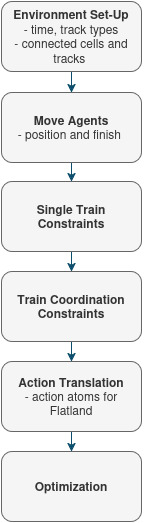
\includegraphics[scale=0.5, width=\linewidth]{base_encoding.jpg}
	\caption{High-level overview of Base Encoding.}
	\label{overview_primary}
\end{wrapfigure}

\subsubsection{Move Agents}
The \verb|position(ID, CELL, TIME, DIRECTION)| argument handles the position of a train (ID) in the environment and thus generates the sequential moves of that agent. A train is marked as \verb|finish(ID, TIME)| once it has reached its destination and doesn't move further. The position atoms are subsequently translated to action predicates containing necessary information, namely train ID and the required action at a given time step, for Flatland to visualise the solved environment.

Our optimization objectives encourage trains to reach their destination as soon as possible and prefer one consecutive waiting period over repeated stop-and-go behaviour.

\subsubsection{Constraints}
We implemented two types of constraints on agent movements: single train constraints and train coordination constraints. Single train constraints ensure that a train behaves normally. They forbid u-turns, multiple positions of one agent in the environment and correct finishing upon arrival at the destination.

Train Coordination constraints avoid behaviour that would cause collisions between agents. Any two given trains cannot occupy the same cell and two oncoming agents cannot immediately switch places or pass through each other.


\subsection{Python Part}\label{solve}
\subsubsection{Track Malfunction Implementation}

Since we could not implement track malfunctions directly in Flatland, we implemented them in Python code that runs Clingo with Flatland input (\verb|solve.py|).

The added code consists of multiple parts:

\begin{itemize}
    \item Creating track malfunctions either randomly or deterministically
    \item Translating the track malfunction Python object into Clingo
    \item Forwarding the atoms to Clingo
    \item Logging the malfunction in a file
    \item Depicting the malfunction in the Flatland output
\end{itemize}

\subsubsection{How is a track malfunction created?}

A track malfunction Python object is a tuple consisting of three components:

\begin{verbatim}
(cell, timestep, duration)
\end{verbatim}

The \texttt{cell} is an \texttt{(X, Y)} tuple that defines where the track malfunction occurred.

The \texttt{timestep} represents the timestep at which the track malfunction was triggered. During this timestep, the malfunction has not yet occurred; it starts in the following timestep. This was an architectural decision to ensure that trains cannot be on a malfunctioning track when the malfunction starts.

The \texttt{duration} specifies the number of timesteps for which the track malfunction occurred.

Track malfunctions can either be created randomly or predefined by the user. The variable \texttt{predefined\_malfunction} is used to store malfunctions that the user wants to enforce on the environment. If the variable is empty, there is a 1\% chance of a malfunction occurring at every timestep (this probability can be adjusted). In the current setup, only one malfunction can occur per timestep. \textbf{(Improvement idea)}

\subsubsection{How is a malfunction implemented in Clingo?}\label{fwd_info_2_clingo}

When a malfunction is triggered in Python, multiple atoms and rules are generated and forwarded to the program that calculates the rescheduling (secondary encoding - see Section \ref{encoding_2}).

\begin{itemize}
    \item \textbf{\texttt{action} constraint rules} -- To preserve the actions taken up to this point, a constraint rule is generated for each action, ensuring that all past actions must be present in the output of the rescheduling.

    \item \textbf{\texttt{track\_malfunction} atoms} -- Used to provide the timestep and duration of the malfunction.

    \item \textbf{\texttt{position} constraint rules} -- Since the track malfunction starts one timestep after it is triggered, the actions at the time the malfunction is triggered are preserved. Consequently, their positions in the next timestep are also preserved. These constraints only include the next position.

    \item \textbf{\texttt{planned\_action} atoms} -- Include all actions that were planned before the malfunction occurred.

    \item \textbf{\texttt{planned\_position} atoms} -- Include all positions that were planned before the malfunction occurred.

    \item \textbf{\texttt{current\_position} atoms} -- Include all positions occupied at the timestep at which the malfunction occurred.
\end{itemize}

\subsubsection{How is the malfunction logged?}

The malfunction is logged in a CSV file with the following parameters:

\begin{verbatim}
timestep;cell;duration
\end{verbatim}


\subsubsection{How is the malfunction depicted?}

Similar to a train malfunction, a track malfunction is depicted as a red \textbf{X} over the malfunctioning track.


\subsection{Secondary Encoding} \label{encoding_2}
The secondary encoding reschedules the environment after a track malfunction. It has Our goal was to reduce computational cost by avoiding recalculation of the environment and agents. Our approach, similar to Gilkra2025 \cite{gilkra2025}, reuses information and train schedules from the original plan unless the track malfunction interferes with an agent. 

\verb|secondary_encoding.lp| reuses ideas for solving from the base encoding, such as the general environment facts \verb|connections_nswe.lp| and \verb|trainjacent| atoms for finding valid movements (see Section \ref{setup_base}). Additionally, information is passed from the original schedule (see Section \ref{fwd_info_2_clingo}). Thus, the secondary encoding has access to 
\begin{itemize}
	\item basic Flatland information (\verb|connections_nswe.lp|)
	\item details of the track malfunction (\verb|track_malfunction\3|)
	\item agent history (\verb|action| and \verb|position| constraints, \verb|current_position\4|)
	\item initial plan for agents (\verb|planned_action\3|, \verb|planned_position\4|)
\end{itemize}


First, the program sets up the required environment with \verb|connections_nswe.lp| and creates two time counters. \verb|time(T)| counts time from one step after the track malfunction. \verb|past_time(T)| counts time up until and including the step of the track malfunction. This distinction is required to restore actions up until the malfunction time. These action atoms are necessary for Flatland to depict the solution correctly.

If a track malfunction triggers before all trains of the environment have been initialized in their starting position, they have to be positioned during rescheduling. Then the replanning of trains starts. There are three scenarios our secondary encoding handles: a) the track malfunction doesn't interfere with the planned routes of agents (no consequence), b) one train is affected by the track malfunction (simple consequence) and c) multiple trains are affected by the track malfunction (complex consequence).

\subsubsection{No Consequence}

\subsubsection{Simple Consequence (no collision)}
\subsubsection{Complex Consequence (collision/ multi-agent rescheduling)}
\subsubsection{create accidents}

\section{Experiments}
\subsection{Rescheduling Methods}

We assume that most of the non-solving time is used to ground the rules.
The objective of each method is described below.

\subsection{Difference in Output of Reschedule Malfunction}

The output for each method when rescheduling after a malfunction will not
necessarily be the same. The base encoding and the secondary encoding with
time prioritization will output the optimal solution, meaning that the trains
will spend the least possible amount of time on the network overall.

However, the secondary encoding with and without heuristics prioritizes the
preservation of the planned schedule. This means that even if delaying a
non-consequent train would improve the overall travel time, only the base
encoding and the secondary encoding with time prioritization will derive this
solution. The other two methods will not be able to choose this solution.

\subsection{Grounding Time}

The grounding time is similar for all methods and, even for larger
environments, usually does not account for more than 10\% of the total
running time.

When the malfunction occurred at the beginning of the schedule, the base
encoding was 30\% faster than the secondary encoding. However, when the
malfunction occurred in the middle of the schedule, the secondary encoding
was 30\% faster.

This can be explained by the fact that, in the base encoding, the positions
and actions for all time steps must be grounded using complex logic. In the
secondary encoding, however, the past and current positions and actions are
already set and do not need to be grounded using the complex rules. Only
future positions and actions need to go through the complex logic.

Therefore, while the logic in the secondary encoding is more complex for
future time steps, some malfunctions can still be grounded faster if the
malfunction occurs late enough in the schedule.

\subsection{Solving Time}

Looking at the solving times, for smaller environments, the running time is
low for all methods. For larger environments, the secondary encoding with
heuristics is always preferable. When the malfunction has no consequences,
solving with the secondary encoding almost always takes less than one
second, even when there is a consequence but no future collision.

For malfunctions that cause a collision, the running times were closer
between the methods, but the secondary encoding still ran 75\% faster than
the base encoding.

Surprisingly, using the base encoding is almost always preferable to using
the secondary encoding without the heuristic flag. We assume that since the
secondary encoding has more rules and options, it is harder to solve.

Comparing the base encoding and the secondary encoding with time
prioritization, the base encoding is faster when there is no consequence,
whereas the secondary encoding with time prioritization is faster when there
is a consequence.

\subsection{Why is Adding the Heuristic Flag Important?}

In the beginning, we implemented the secondary encoding without the heuristic
addition. We were perplexed by the fact that running the environment with
the secondary encoding took more time than with the base encoding.

For us, it was obvious that since most malfunctions either do not affect the
trains or affect only one or two trains, most trains should be able to simply
use the output from the base encoding. However, Clingo still needed to
re-prove that the solution was optimal.

Clingo started with an initial solution that recalculated all the trains and,
after many iterations, eventually reached the original planned solution.

After adding the heuristic flag, Clingo found that most trains should use the
original planned solution already in the first iteration.

\subsection{When to Use Each Method?}

There are two possible goals that a user might want when rescheduling after
a malfunction:

\begin{itemize}
    \item Change the least amount of trains possible, i.e., preserve the
    previous schedule as much as possible.
    \item Obtain the most optimized solution.
\end{itemize}

Both goals should be achieved as quickly as possible.

For the purpose of comparing the methods, we assume that the output of the
initial schedule using the base encoding is already saved. This assumption
reflects the real-world scenario in which the schedule is set in advance and
the malfunction occurs later.

For obtaining the most optimized solution, the base encoding and the
secondary encoding with time prioritization are the preferred methods. Conversely, 
the secondary encoding with and without heuristics are used to produce 
an answer with the least amount of changed trains.

For smaller environments, defined as a height below 20, a
width below 20, and fewer than 3 trains, all methods are very fast, and no
malfunction requires more than 5 seconds to find a solution.

For larger environments, however, the differences between the methods become
significant. If the user wants to obtain the least amount of changed trains
possible, they should choose the secondary encoding with heuristics, as it is
consistently the fastest method, often by a large margin.

If the user wants the most optimized solution, the preferred method depends
on whether there is a consequence. If there is a consequence, the secondary
encoding with time prioritization is the better choice in most cases.
Otherwise, the base encoding is faster.

Combining all the conclusions derived above, we can create a flow that
describes how to handle a malfunction. First, the secondary encoding is run
to derive Solution A. If there is no consequence, Solution A is both the most
optimized solution and the solution with the least amount of changed trains.
If there is a consequence, the appropriate solution depends on the user's
goal. If the goal is to minimize the number of changed trains, Solution A can
be used directly. If the goal is to obtain the most optimized solution, the
secondary encoding with time optimization is run to derive Solution B.
Most malfunctions will not have a consequence, so it is better to run the
secondary encoding first and determine whether rescheduling is necessary.
The secondary encoding is also very fast in all cases, so an answer will be
available before the other methods.

Using the secondary encoding with time optimization only when a consequence
is detected was faster than the base encoding in all tested cases.

The following graph depicts which method should be used based on the desired
output:
\begin{figure}[ht]
    \centering
    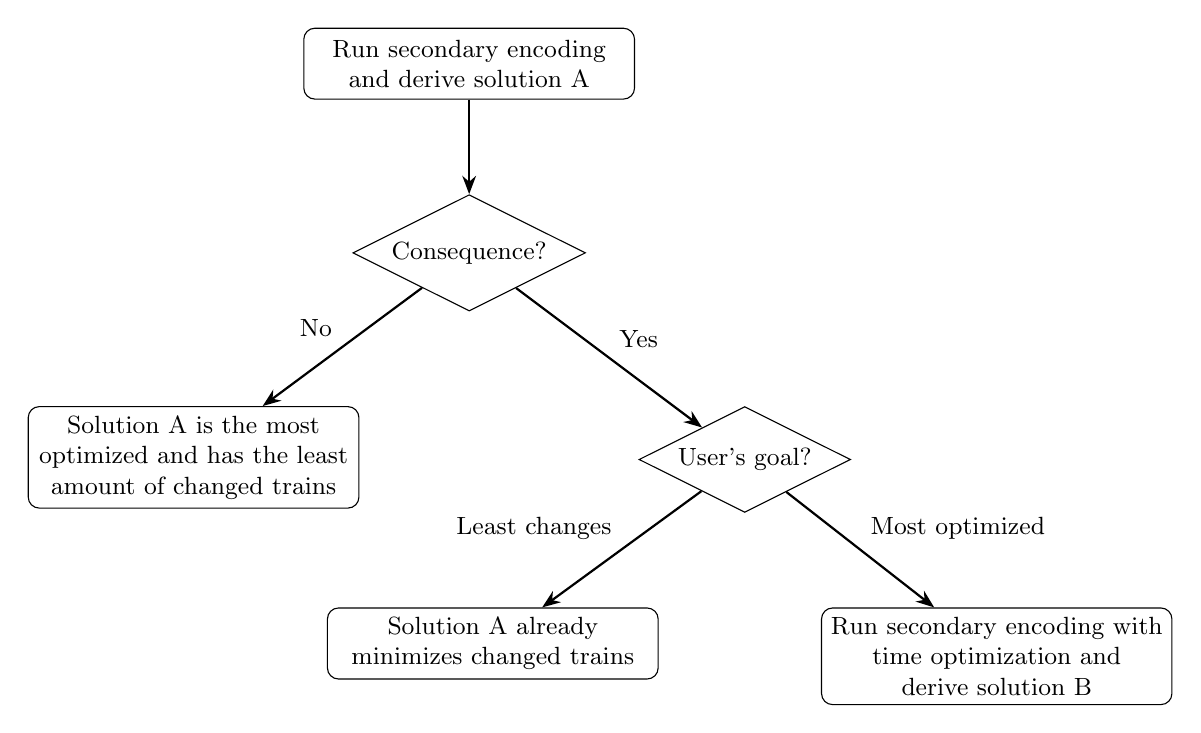
\begin{tikzpicture}[
        node distance=1.2cm,
        every node/.style={font=\small},
        process/.style={
            rectangle,
            rounded corners,
            draw,
            align=center,
            minimum width=4.2cm,
            minimum height=0.9cm
        },
        decision/.style={
            diamond,
            draw,
            align=center,
            aspect=2,
            inner sep=2pt
        },
        arrow/.style={
            -{Stealth},
            thick
        }
    ]

    % Start
    \node[process] (start)
        {Run secondary encoding\\
         and derive solution A};

    % First decision
    \node[decision, below=of start] (consequence)
        {Consequence?};

    % No consequence branch
    \node[process, below=of consequence, xshift=-3.5cm] (no)
        {Solution A is the most\\
         optimized and has the least\\
		 amount of changed trains};

    % Consequence branch
    \node[decision, below=of consequence, xshift=3.5cm] (goal)
        {User's goal?};

    % Least changed trains
    \node[process, below=of goal, xshift=-3.2cm] (least)
        {Solution A already\\
         minimizes changed trains};

    % Most optimized
    \node[process, below=of goal, xshift=3.2cm] (optimized)
        {Run secondary encoding with\\
         time optimization and\\
		 derive solution B};

    % Arrows from start
    \draw[arrow] (start) -- (consequence);

    % Consequence branches
    \draw[arrow] (consequence)
        -- node[above left] {No} (no);

    \draw[arrow] (consequence)
        -- node[above right] {Yes} (goal);

    % User goal branches
    \draw[arrow] (goal)
        -- node[above left] {Least changes} (least);

    \draw[arrow] (goal)
        -- node[above right] {Most optimized} (optimized);

    \end{tikzpicture}
    \caption{Decision process for selecting a rescheduling method.}
    \label{fig:rescheduling-method-selection}
\end{figure}

\subsection{compare grounding for two versions of trains can't be in same cell at same time rule}

\section{Log / Timeline}

\begin{itemize}
	\item merge encodings (May 29)
	\item literature review zank2026, gilkra2025a, waldow2025a (June 6)
	\item fix visualization issue aka add wait before start time (June 9)
	\item "crack the egg" pkl-file (June 17)
	\item understand solve.py (June 18)
	\item create pipeline for track malfunction in parallel to train malfunction TrackMalManager etc. (June 22)
	\item pick relevant track for malfunction randomly (July 2)
	\item create visualization for track malfunction ()
	\item create track malfunction log (July 13)
	\item start secondary encoding (no consequence or rescheduling necessary) (July 14)
	\item expand secondary encoding: handle rescheduling of directly affected train (August 2)
	\item finish secondary encoding: handle collisions due to rescheduling (August 3)
	\item improve encodings: minimize grounding, remove unnecessary rules (August 7)
	\item add heuristic, code cleaning and remove can\_dir (August 10)
	\item separate predefined and random track malfunctions, code clean-up (August 13)
\end{itemize}

\section{Future Work}
\begin{itemize}
	\item explore options instead of random malfunctions (frequented tracks, crosses, etc.)
	\item explore option of tertiary encoding (recalculate from scratch if malfunction hits early on: first > secondary > first)
	\item heuristic assumes loose rail network BUT not realistic (maybe discussion part)
	\item handle unsatisfiable as a result of calculating after malfunction (?)
\end{itemize}

\section{Experiment 1}
We compared the use of the secondary encoding with rescheduling the entire environment anew with the base encoding. For this, we have created four testing environments of varying sizes (2 small and 2 medium environments - see Figure \ref{test_envs}). In each environment we have identified tracks for all three types of track malfunctions (simple, complex, no consequence - see Section \ref{encoding_2}). We ran each environment and malfunction in two modes. Mode 1-1 scheduled and rescheduled with the base encoding. 1-2 used the base encoding only for scheduling and the secondary encoding for rescheduling. 

\begin{figure}[hbt!]
	
	\begin{subfigure}{.475\linewidth}
		
\includegraphics[width=\linewidth]{environment.png}
		\caption{}
		\label{MLEDdet}
	\end{subfigure}\hfill % <-- "\hfill"
	~ % optional tilde b/t figures for readability.
	% this solution will not work w/ empty lines b/t subfigures
	\begin{subfigure}{.475\linewidth}
		
\includegraphics[width=\linewidth]{environment.png}
		\caption{}
		\label{energydetPSK}
	\end{subfigure}
	
	\medskip % create some *vertical* separation between the graphs
	\begin{subfigure}{.475\linewidth}
		
\includegraphics[width=\linewidth]{environment.png}
		\caption{}
		\label{velcomp}
	\end{subfigure}\hfill % <-- "\hfill"
	% or just a comment and no tilde
	\begin{subfigure}{.475\linewidth}
		
\includegraphics[width=\linewidth]{environment.png}
		\caption{}
		\label{velqual}
	\end{subfigure}
\caption{These are the testing environments.}
\label{test_envs}
\end{figure}

\begin{table}[h!]
	\centering
	\begin{tabular}{|l|l|l|r|r|}
		\hline
		Env name & Mal type & Mode & Schedule & Reschedule  \\ \hline
		\textbf{env\_016} & simple & 1-2 & 0.092 & 0.084 \\ \hline
		{} & simple  & 1-1 & 0.095 & 0.082  \\ \hline
		{} & complex & 1-2 & 0.097 & 0.070 \\ \hline
		{} & complex & 1-1 & 0.092 & 0.089 \\ \hline
		{} & no cons & 1-2 & 0.185 & 0.116 \\ \hline
		{} & no cons & 1-1 & 0.100 & 0.107 \\ \hline
		\textbf{env\_028} & simple & 1-2 & 0.114 & 0.038 \\ \hline
		{} & simple & 1-1 & 0.057 & 0.047  \\ \hline
		{} & complex & 1-2 & 0.057 & 0.056 \\ \hline
		{} & complex & 1-1 & 0.057 & 0.055 \\ \hline
		{} & no cons & 1-2 & 0.065 & 0.050 \\ \hline
		{} & no cons & 1-1 & 0.065 & 0.061 \\ \hline
		\textbf{env\_033} & simple & 1-2 & 0.651 & 0.389 \\ \hline
		{} & simple & 1-1 & 0.583 & 0.607 \\ \hline
		{} & complex & 1-2 & 0.589 & 0.867 \\ \hline
		{} & complex & 1-1 & 0.598 & 3.747 \\ \hline
		{} & no cons & 1-2 & {} & {}  \\ \hline
		{} & no cons & 1-1 & {} & {} \\ \hline
		\textbf{env\_035} & simple & 1-2 & 26.135 & 2.116 \\ \hline
		{} & simple & 1-1 & 26.240 & 11.449 \\ \hline
		{} & complex & 1-2 & 26.299 & 2.053 \\ \hline
		{} & complex & 1-1 & 26.251 & 35.805 \\ \hline
		{} & no cons & 1-2 & 26.471 & 6.579  \\ \hline
		{} & no cons & 1-1 & 26.219 & 22.771 \\ \hline
		
	\end{tabular}
\vspace{0.2cm}

	\begin{tabular}{|l l|}
		\hline
		1-1: & base encoding for scheduling and rescheduling \\
		1-2: & base encoding for scheduling, secondary encoding for rescheduling\\ \hline
	\end{tabular}

\vspace{0.2cm}

\caption{Results for testing environments with different malfunction types.}
\label{encodings}
\end{table}

\section{Discussion}


%
% ---- Bibliography ----
%
% BibTeX users should specify bibliography style 'splncs04'.
% References will then be sorted and formatted in the correct style.
%
\bibliographystyle{splncs04}
\bibliography{refs}
%%
%\begin{thebibliography}{8}
%\bibitem{ref_article1}
%Author, F.: Article title. Journal \textbf{2}(5), 99--110 (2016)
%
%\bibitem{ref_lncs1}
%Author, F., Author, S.: Title of a proceedings paper. In: Editor,
%F., Editor, S. (eds.) CONFERENCE 2016, LNCS, vol. 9999, pp. 1--13.
%Springer, Heidelberg (2016). \doi{10.10007/1234567890}
%
%\bibitem{ref_book1}
%Author, F., Author, S., Author, T.: Book title. 2nd edn. Publisher,
%Location (1999)
%
%\bibitem{ref_proc1}
%Author, A.-B.: Contribution title. In: 9th International Proceedings
%on Proceedings, pp. 1--2. Publisher, Location (2010)

%\bibitem{ref_url1}
%LNCS Homepage, \url{http://www.springer.com/lncs}, last accessed 2023/10/25
%
%\bibitem{flatlandpaper}
%Mohanty et. al: Flatland-RL: Multi-Agent Reinforcement Learning on Trains. \url{https://arxiv.org/abs/2012.05893}, 2020.
%
%
%\end{thebibliography}
\end{document}
